\documentclass{article}
\usepackage[utf8]{inputenc}
\usepackage{amsmath, amssymb}
\usepackage{graphicx}
\usepackage{array}
\usepackage[margin=1in]{geometry}
\usepackage[slovenian]{babel}
\usepackage{caption}
\usepackage{subcaption}
\usepackage{tabularx}
\usepackage{siunitx}
\sisetup{locale = SI}
\sisetup{input-decimal-markers = {,}, output-decimal-marker = {,}}

\title{LAB03: SILE IN NABOJI}
\author{Sinja Kortnik, Simon Sovič, Marko Gjurovski} 
\date{22. 10. 2026}

\begin{document}
\maketitle

\section{Aplikativni poskus}
a: Najprej naelektrimo obe krogli. Eno postavimo na tehtnico, drugo pa držimo nad njo, kakor je prikazano na skici (slika \ref{skica1}). 
Opazujemo kako se spremeni masa krogle na tehtnici. Najprej poskus izvedemo z enako nabitima kroglama, potem ga 
ponovimo z nasprotno nabitima. Če se prikazana masa zmanjša se krogli privlačita, torej sta nabiti z nasprotnim 
nabojem, če se poveča, pa se odbijata, torej sta nabiti z enakim nabojem. Tako pokažemo, da sta krogli naelektreni. 
To ponovimo, vendar namesto druge krogle uporabimo palico, za katero vemo, kakšen je njen naboj. Ponovno opazujemo, 
ali se masa poveča ali zmanjša. Tako potrdimo, da je na palici enak naboj kot na krogli. \\
b: 
\begin{enumerate}
  \item Ko nabijemo obe krogli s stekleno palico, po kateri drgnemo s svilo, se masa na tehtnici poveča za $m = \SI{0,21\pm 0,01}{g}$, kar pomeni, da 
se krogli odbijata. 
  \item Ko nabijemo obe krogli s plastično palico, po kateri drgnemo s krznom, se masa na tehtnici poveča za $m = \SI{0,5\pm 0,01}{g}$, kar pomeni, da
se krogli odbijata. 
  \item Ko pa eno kroglo nabijemo s plastično palico, po kateri drgnemo s krznom in drugo s stekleno palico, po kateri drgnemo s svilo, 
se masa na tehtnici zmanjša za $m = \SI{0,3 \pm 0,01}{g}$, kar pomeni, da se krogli privlačita. 
  \item Ko nabijemo eno kroglo s plastično palico, po kateri drgemo s krznom in ji približamo enako palico, se masa na tehtnici
poveča, kar pomeni, da se krogla in palica odbijata. Tako dokažemo, da imata enak naboj. 
Enako se zgodi tudi za stekleno palico, po kateri drgnemo s svilo. 
\end{enumerate}
c: Da.
\begin{figure}[h!]
  \centering
  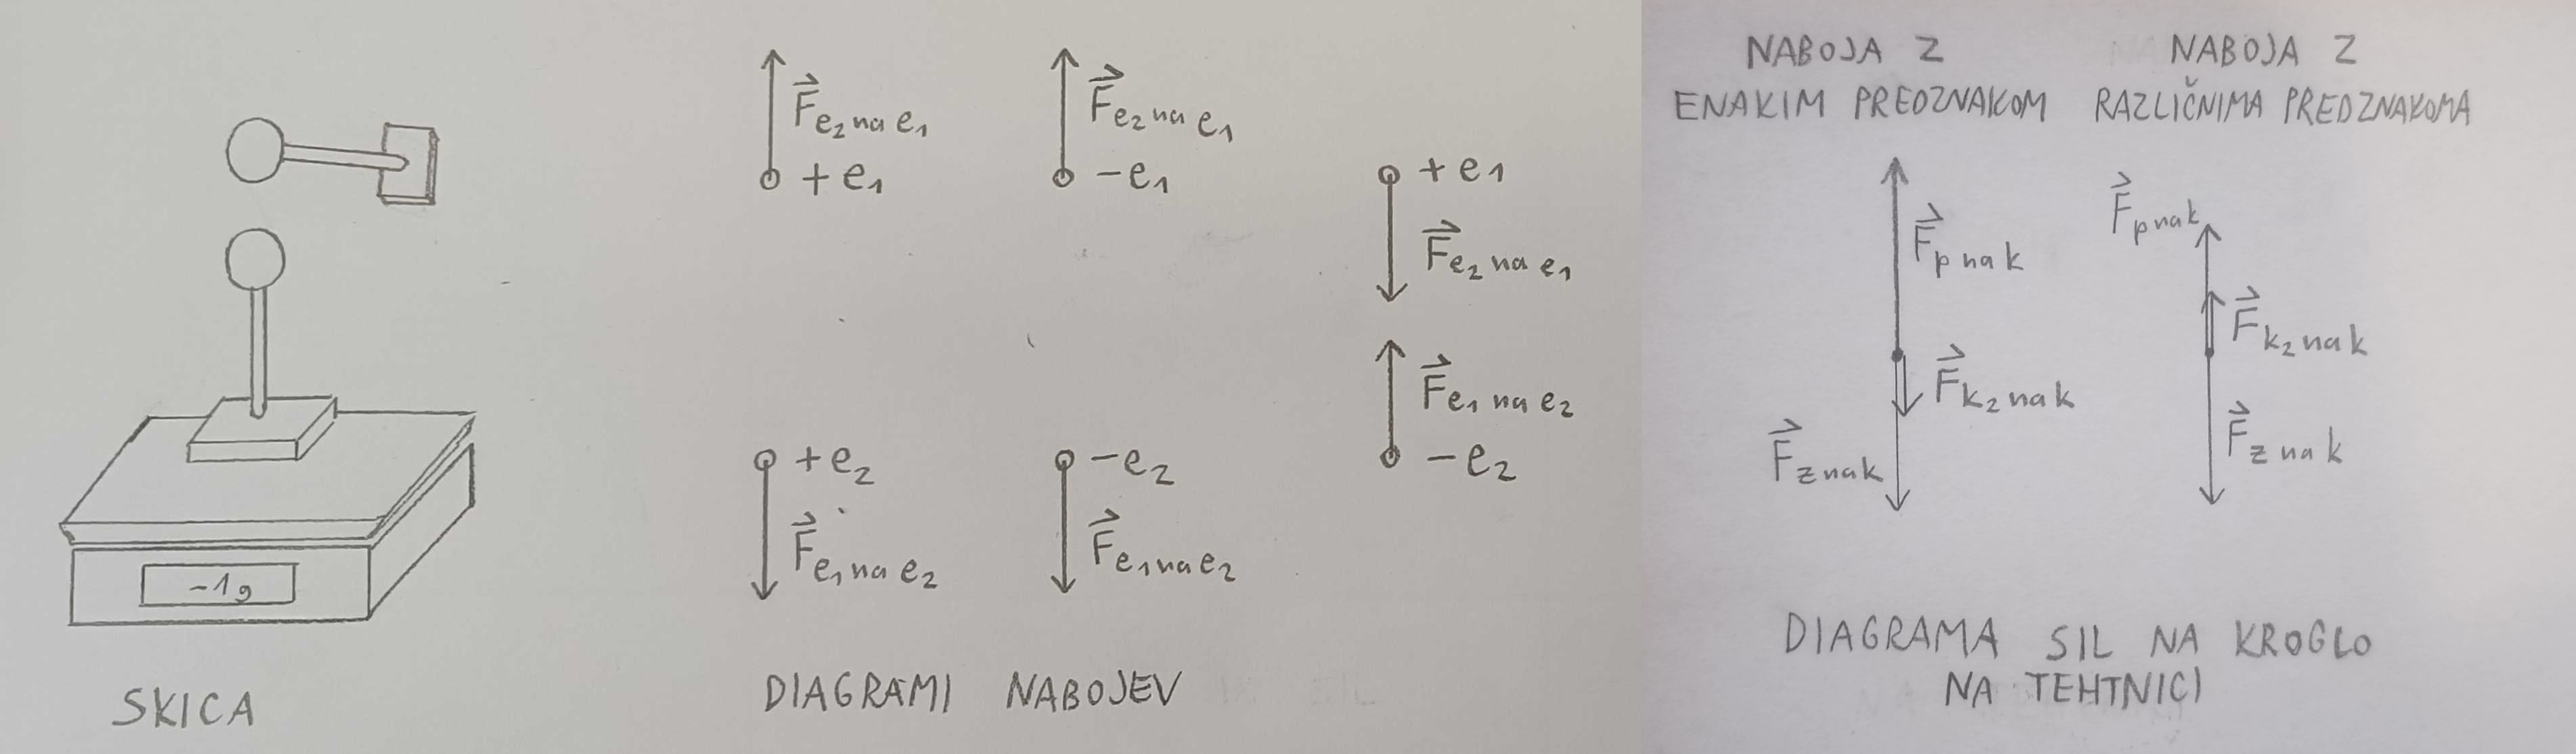
\includegraphics[width=\linewidth]{popravljeno1.jpg}
  \caption{Skica postavitve poskusa, diagram nabojev in diagram sil za kroglo na tehtnici.}
   \label{skica1}
\end{figure}


\section{Dva opazovalna poskusa}

\subsection{Prvi opazovalni poskus}
a, b in c: Začetna masa na tehtnici je bila $m_0 = \SI{76,26\pm 0,01}{g}$, končna masa pa $m_k = \SI{76,11\pm 0,01}{g}$. 
d: Ko smo naelektreni krogli približali drugo nenaelektreno kroglo, se je v nenaelektreni krogli naboj prerazporedil
(slika \ref{skica2}). Ta pojav imenujemo influenca. V delu bližje negativno naelektreni krogli se je naboj prerazporedil tako, da je 
bil v tem delu pozitiven, v nasprotnem delu pa je bil naboj negativen. Zaradi tega sta se krogli privlačili, 
masa na tehtnici pa se je zmanjšala. \\
\begin{figure}[h!]
  \centering
  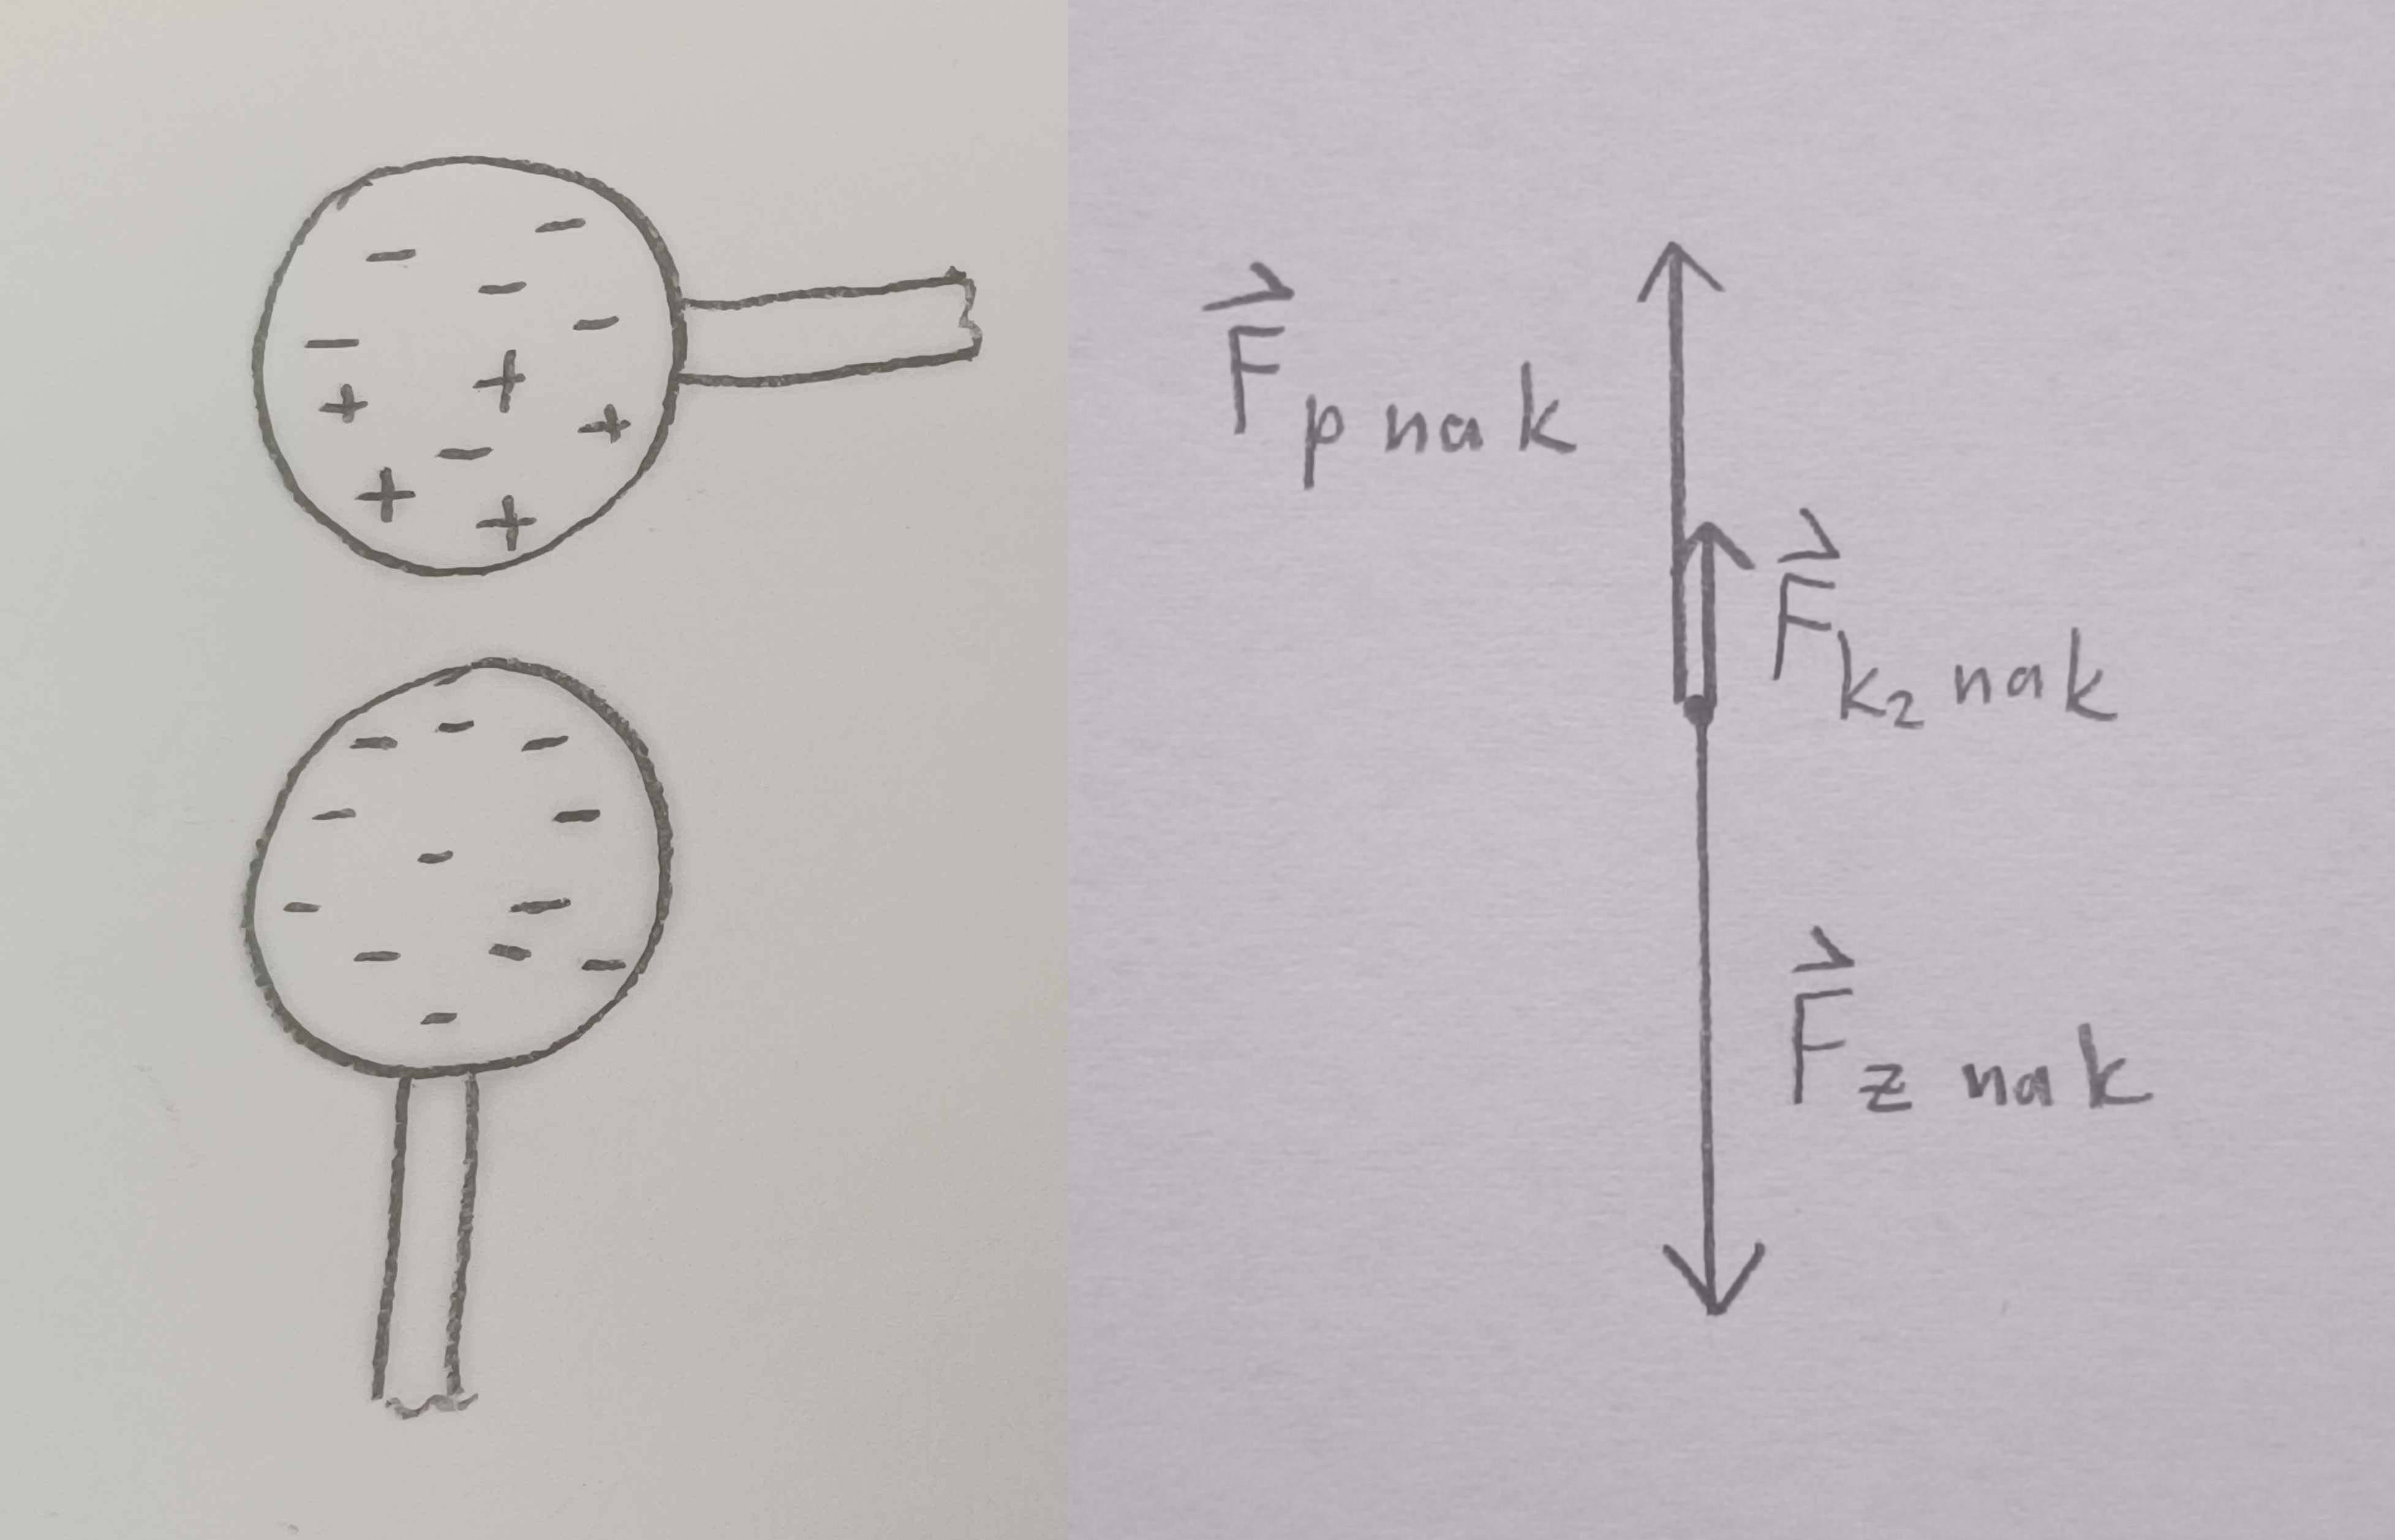
\includegraphics[width=0.5\linewidth]{popravljeno2.jpg}
  \caption{Skica pojava influence in diagram sil za kroglo na tehtnici.}
   \label{skica2}
\end{figure}
e: Izvedemo poskus, kot je prikazan na skici (slika \ref{skica3}). Nad originalno postavitev dodamo še negativno naelektreno palico. Naboj 
se bo ponovno prerazporedil, kakor na skici. Če je predlagana razlaga pravilna in naredimo zgoraj opisan poskus, 
se bo masa na tehtnici povečala,
saj se bo pozitiven naboj prerazporedil na dva konca nevtralne krogle in bo efekt privlačne sile med kroglama manjši. \\
f: Začetna masa je $m_0 = \SI{76,24\pm 0,01}{g}$, ko približamo nevtralno kroglo se zmanjša in je $m_1 = \SI{75,95\pm 0,01}{g}$, ko dodamo
še plastično negativno nabito palico, se masa poveča in je $m_k = \SI{76,10\pm 0,01}{g}$. Da, izid se ujema z našo napovedjo. 
Naša razlaga je pravilna.
\begin{figure}[h!]
  \centering
  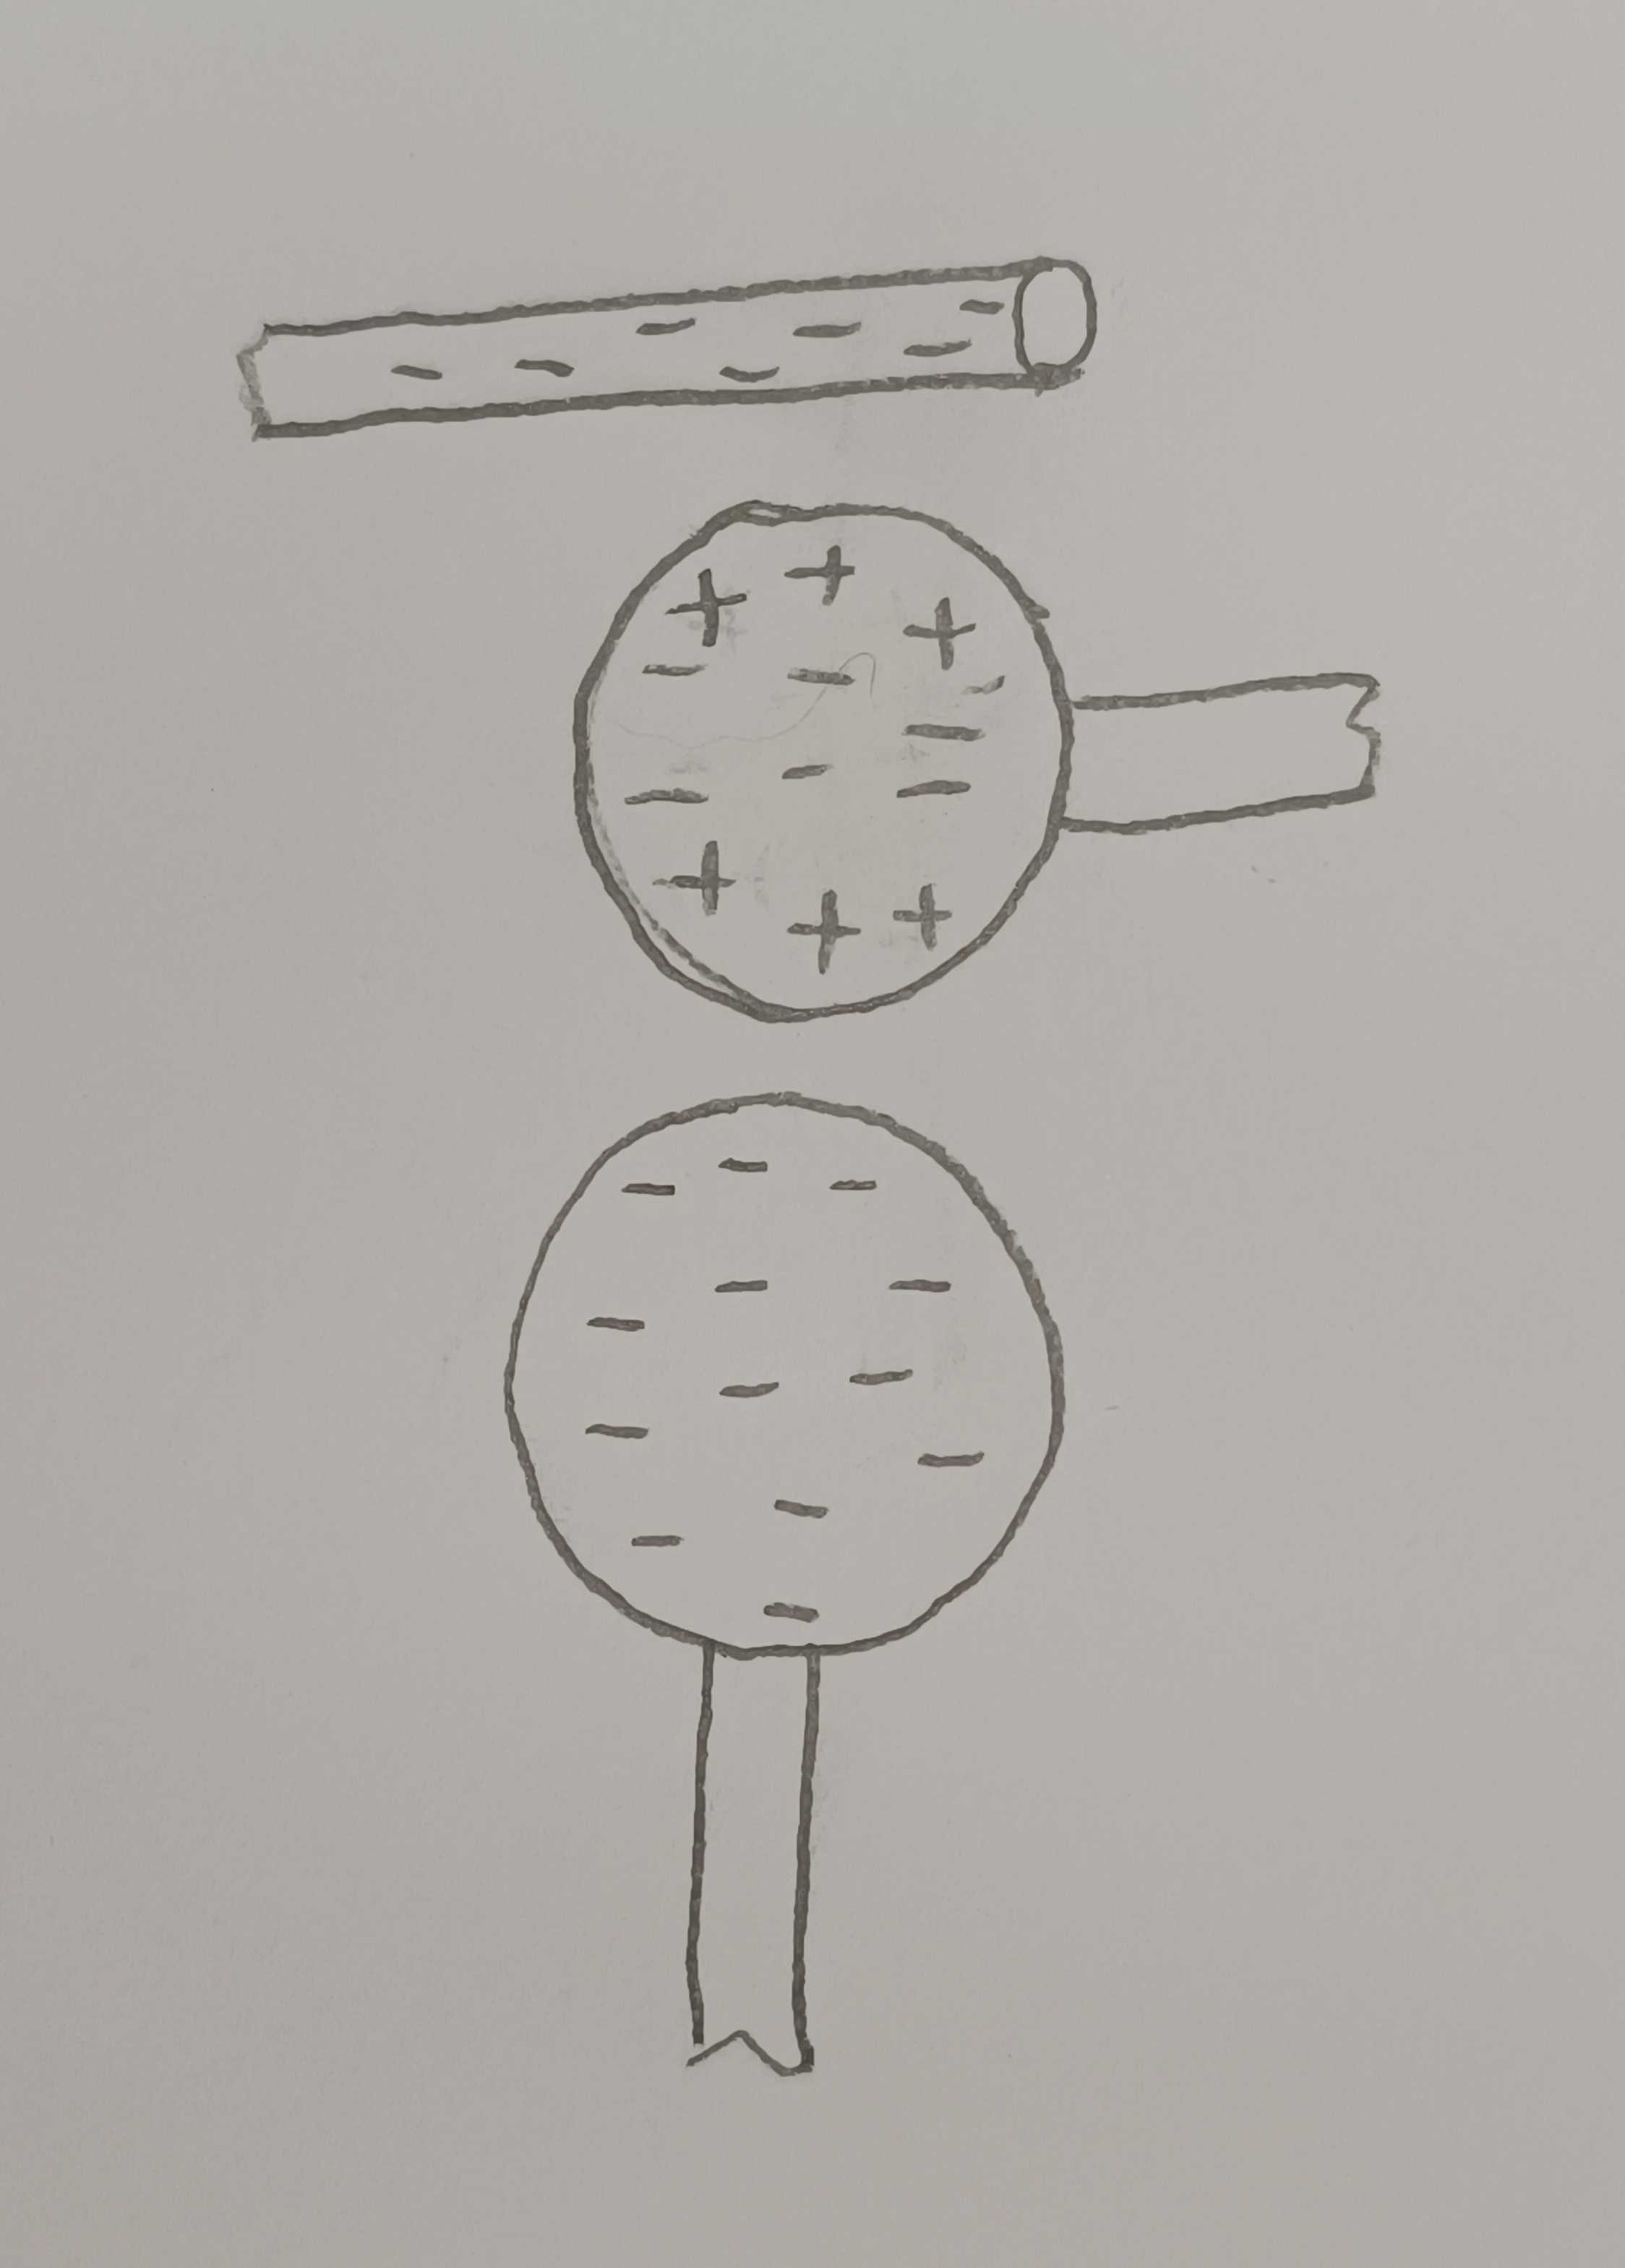
\includegraphics[width=0.3\linewidth]{skica3.jpg}
  \caption{Skica prvega testnega poskusa.}
   \label{skica3}
\end{figure}
\subsection{Drugi opazovalni poskus}
g: Ko približamo nevtralno kroglo negativno nabiti krogli, se masa prvotno zmanjša, kot v prejšnjem opazovalnem
poskusu: $m_0 = \SI{76,24\pm 0,01}{g}$ in $m_1 = \SI{76,20\pm 0,01}{g}$. Nato smo se dotaknili nevtralne krogle s prstom, masa se je ponovno
znižala na $m_k = \SI{76,15\pm 0,01}{g}$. \\
h: Ko se krogle dotaknemo s prstom, se pozitivni naboj iz našega telesa prenese na kroglo ali pa se negativni naboj
iz krogle prenese na naše telo. Prej nevtralna krogla je zdaj rahlo pozitivno nabita. Naboj se razporedi po principu
influence. Ker je zdaj krogla bolj pozitivno nabita, je privlak večji in posledično prikazana masa manjša. \\
i: Ponovimo celoten postopek opisan v točki g. Nato zdaj rahlo pozitivno nabito kroglo odstranimo s stojala in
jo položimo na tehtnico. Približamo ji negativno nabito palico. Kot v prvem poskusu pričakujemo, da se bosta zdaj,
če je krogla res pozitivno nabita, palica in krogla privlačili in se bo posledično masa zmanjšala. \\
j: Masa pozitivne krogle na tehtnici je $m_0 = \SI{76,94\pm 0,01}{g}$. Ko ji približamo negativno nabito palico, se masa zmanjša na
$m_k = \SI{76,89\pm 0,01}{g}$. Rezultat testnega poskusa se ujema z našo razlago.
\begin{figure}[h!]
  \centering
  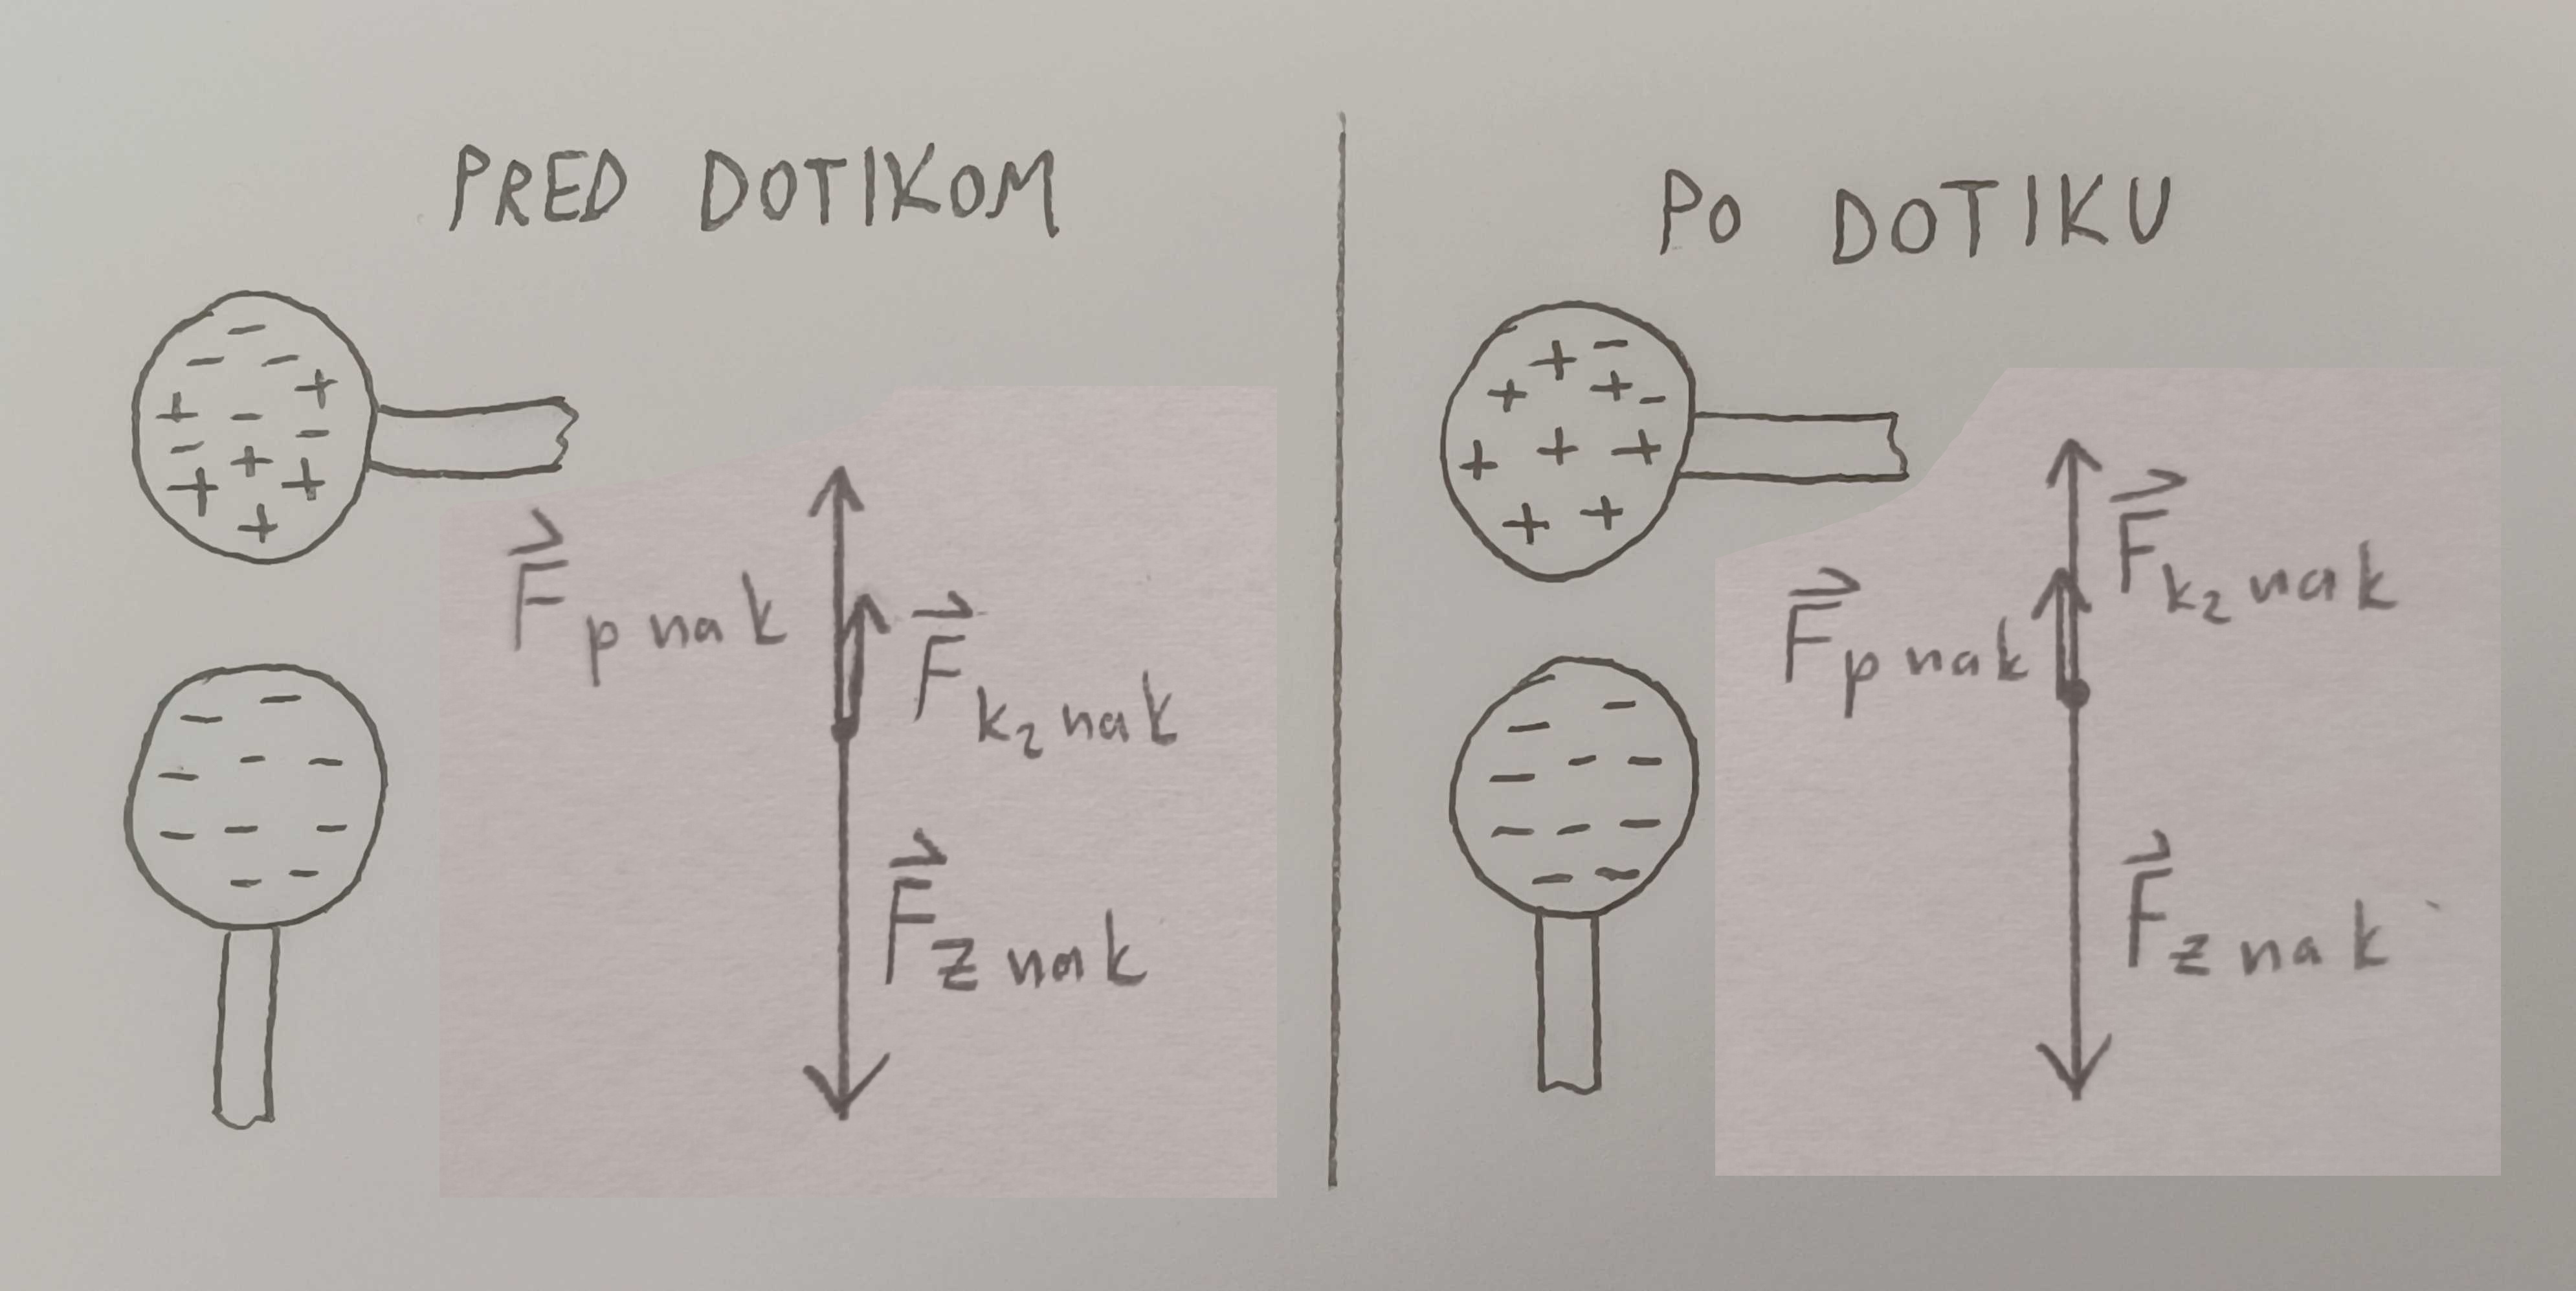
\includegraphics[width=0.5\linewidth]{popravljeno3.jpg}
  \caption{Skica drugega testnega poskusa in diagram sil za kroglo na tehtnici.}
\end{figure}





\end{document}
